\section{Text signal: a supervised technology taxonomy}

\subsection{Why CPV is not enough}

The cohort is defined by four CPV divisions. That is reproducible and auditable --- and coarse: CPV says a procurement is digital, not what was bought. Yet every business question Gigalis asks lives at the second level: which segments are growing, which are re-procured fastest, where to open a framework agreement. This section learns that missing variable from the text of the contract object:

\[\text{procurement object text} \longrightarrow \text{supervised classifier} \longrightarrow \text{business technology class}\]

It is an \textbf{enrichment layer}. It does not replace the CPV segmentation, which remains the cohort definition, the Cox covariate, and the axis of the time series.

\subsection{Taxonomy and corpus}

Eight substantive classes --- cloud/hosting, cybersecurity, network/telecom, IT infrastructure, business software, data/BI, AI and IT services --- plus three fallback classes that are \textbf{annotation decisions}, not missing values: \texttt{MIXED} (no dominant technology), \texttt{OTHER\_DIGITAL} (a digital purchase outside the eight), \texttt{OTHER} (a digital CPV on something that is not a technology purchase). The taxonomy was frozen before any modelling.

The corpus holds \textbf{500 manually annotated notices}, 2015-2025, all with a non-empty object text (median 14 words). Two properties constrain how it may be read. The sample is \textbf{quota-stratified}: the class proportions are a property of the annotation design, not an estimate of prevalence. And the \texttt{AI} class holds only \textbf{7 notices} across eleven years: no synthetic examples were created, no rows duplicated, no oversampling applied. The consequence is published rather than engineered away.

\subsection{Leakage prevention}

The BOAMP republishes procedures, and buyers re-run near-identical consultations a few years apart. Scoring a model on a near-copy of a document it trained on measures memorisation. Every notice is therefore assigned to a \textbf{procurement family}, defined as the union of two rules: notices already grouped into one reconstructed episode, and notices whose objects reach a character-level cosine similarity of 0.80. Each family belongs to exactly one fold.

The second rule is not redundant: the first alone gives 486 groups; adding the second merges 39 near-duplicate pairs, of which \textbf{29 sit in different episodes} and would otherwise have been split across folds. The result is \textbf{459 families}, none spanning two folds.

One side effect deserves mention: \textbf{3 families contain notices with near-identical text but different labels} --- videoconference services labelled \texttt{NETWORK\_TELECOM} in 2017 and \texttt{OTHER\_DIGITAL} in 2021; an infrastructure-as-a-service procurement labelled \texttt{MIXED} in 2017 and \texttt{CLOUD\_HOSTING} in 2021. No label was changed: no evidence decides which reading is right, and editing labels after seeing the model's errors is how a corpus is fitted to its classifier. They are recorded as an empirical floor on attainable accuracy.

\subsection{Representation and models}

The input is the \texttt{objet} field alone. Normalisation is deliberately light --- mojibake repair, NFC, lowercasing, whitespace --- and \textbf{accents are preserved}, with no stemming: the classes are distinguished by words such as \emph{cybersécurité}, \emph{logiciel métier} and \emph{intelligence artificielle}, and flattening French orthography would discard the evidence. Features are TF-IDF word n-grams \citep{salton1988}; both unigrams and unigrams-plus-bigrams were in the search space, and \textbf{every fold selected unigrams alone}, the bigram vocabulary being too sparse across 500 short documents.

Excluded from the features by design: buyer identity, geography, dates, amounts, procedure type, framework status, notice identifiers, every linkage variable, and CPV --- which serves as the comparator.

Six specifications were compared on identical folds, with hyperparameters selected by inner cross-validation \emph{inside each training fold}:

\begingroup\footnotesize
\begin{longtable}[]{@{}llr@{}}
\toprule\noalign{}
Model & Features & Out-of-fold macro-F1 \\
\midrule\noalign{}
\endhead
\bottomrule\noalign{}
\endlastfoot
Majority class & --- & 0.027 \\
CPV only & CPV codes & 0.441 \\
CPV + BOAMP descriptors & administrative & 0.473 \\
TF-IDF + logistic regression & text & 0.670 \\
\textbf{TF-IDF + class-weighted logistic regression} & text & \textbf{0.744} \\
TF-IDF + linear SVM & text & 0.718 \\
TF-IDF + class-weighted linear SVM & text & 0.715 \\
\end{longtable}
\endgroup

\subsection{The headline result}

\begingroup\small
\begin{longtable}[]{@{}
  >{\raggedright\arraybackslash}p{(\columnwidth - 4\tabcolsep) * \real{0.3000}}
  >{\raggedleft\arraybackslash}p{(\columnwidth - 4\tabcolsep) * \real{0.4000}}
  >{\raggedright\arraybackslash}p{(\columnwidth - 4\tabcolsep) * \real{0.3000}}@{}}
\toprule\noalign{}
\begin{minipage}[b]{\linewidth}\raggedright
Comparison
\end{minipage} & \begin{minipage}[b]{\linewidth}\raggedleft
Macro-F1
\end{minipage} & \begin{minipage}[b]{\linewidth}\raggedright
95 \% CI (family bootstrap)
\end{minipage} \\
\midrule\noalign{}
\endhead
\bottomrule\noalign{}
\endlastfoot
TF-IDF + class-weighted logistic regression & \textbf{0.7442} & {[}0.682; 0.791{]} \\
Best CPV / descriptor comparator & 0.4731 & {[}0.413; 0.526{]} \\
\textbf{Paired difference} & \textbf{+0.2711} & \textbf{{[}0.201; 0.340{]}} \\
\end{longtable}
\endgroup

The interval on the difference excludes zero. Three precautions make this result solid rather than trivial: both sides use \textbf{the same folds} and \textbf{the same hyperparameter search budget}; the difference is \textbf{paired} fold by fold; and the bootstrap resamples \textbf{procurement families}, the unit at which dependence exists, rather than notices.

In other words, the text of the notices carries business information the administrative vocabulary does not. The crosswalk makes this concrete:

\begingroup\footnotesize
\begin{longtable}[]{@{}
  >{\raggedright\arraybackslash}p{(\columnwidth - 8\tabcolsep) * \real{0.1765}}
  >{\raggedright\arraybackslash}p{(\columnwidth - 8\tabcolsep) * \real{0.1765}}
  >{\raggedleft\arraybackslash}p{(\columnwidth - 8\tabcolsep) * \real{0.2353}}
  >{\raggedleft\arraybackslash}p{(\columnwidth - 8\tabcolsep) * \real{0.2353}}
  >{\raggedright\arraybackslash}p{(\columnwidth - 8\tabcolsep) * \real{0.1765}}@{}}
\toprule\noalign{}
\begin{minipage}[b]{\linewidth}\raggedright
CPV division
\end{minipage} & \begin{minipage}[b]{\linewidth}\raggedright
Dominant class
\end{minipage} & \begin{minipage}[b]{\linewidth}\raggedleft
Dominant count
\end{minipage} & \begin{minipage}[b]{\linewidth}\raggedleft
Purity
\end{minipage} & \begin{minipage}[b]{\linewidth}\raggedright
Other classes $\ge$ 100 episodes
\end{minipage} \\
\midrule\noalign{}
\endhead
\bottomrule\noalign{}
\endlastfoot
CPV-32 (telecoms) & Network/telecom & 426 / 1,152 & 0.370 & Other digital 202; business software 146; IT infrastructure 128 \\
CPV-35 (security) & Network/telecom & 165 / 564 & 0.293 & Other 114; cybersecurity 106 \\
CPV-48 (software) & Business software & 348 / 790 & 0.441 & --- \\
CPV-72 (IT services) & IT services & 325 / 1,294 & 0.251 & Business software 310; network/telecom 204; other digital 165 \\
\end{longtable}
\endgroup

Two readings. The mean purity of a CPV segment against the learnt taxonomy is \textbf{0.34}: no division corresponds to a technology. And the largest division, CPV-72, is the least pure of the four (0.251): what the administrative vocabulary calls ``IT services'' in fact spans four business families of comparable size. One telling detail: CPV-32 and CPV-35, two distinct divisions of the vocabulary, share the \textbf{same} dominant predicted class.

\subsection{What the classifier can and cannot do}

\begingroup\footnotesize
\begin{longtable}[]{@{}lrrrr@{}}
\toprule\noalign{}
Class & Precision & Recall & F1 & Support \\
\midrule\noalign{}
\endhead
\bottomrule\noalign{}
\endlastfoot
DATA\_BI & 0.923 & 0.828 & \textbf{0.873} & 29 \\
OTHER & 0.923 & 0.800 & 0.857 & 15 \\
BUSINESS\_SOFTWARE & 0.798 & 0.898 & 0.845 & 88 \\
NETWORK\_TELECOM & 0.810 & 0.840 & 0.824 & 81 \\
CYBERSECURITY & 0.848 & 0.722 & 0.780 & 54 \\
IT\_SERVICES & 0.778 & 0.757 & 0.767 & 74 \\
IT\_INFRASTRUCTURE & 0.702 & 0.717 & 0.710 & 46 \\
OTHER\_DIGITAL & 0.655 & 0.679 & 0.667 & 53 \\
AI & 0.800 & 0.571 & \emph{0.667} & \textbf{7} \\
CLOUD\_HOSTING & 0.731 & 0.594 & 0.655 & 32 \\
MIXED & 0.482 & 0.619 & 0.542 & 21 \\
\end{longtable}
\endgroup

Macro-F1 0.741 (fold standard deviation 0.034), weighted F1 0.765, accuracy 0.766. Two aggregations coexist and should be kept apart: 0.741 is the \textbf{mean across the three folds}, whereas the headline figure of \S~6.5, 0.744, is computed \textbf{out of fold on the pooled 500 predictions}. The gap is the expected one between an average of per-fold scores and a single score over all predictions.

Three readings. The reliable classes are \texttt{CYBERSECURITY}, \texttt{NETWORK\_TELECOM}, \texttt{BUSINESS\_SOFTWARE}, \texttt{DATA\_BI}, \texttt{IT\_SERVICES} and \texttt{OTHER}. \texttt{MIXED} is weak, which is consistent with its definition as the bucket for procurements without a dominant technology. And \textbf{\texttt{AI} is not interpretable}: its F1 of 0.667 rests on three correct predictions; a high number would be a small-sample artefact and a low one equally uninformative.

Error analysis on thirty representative cases gives: 16 model errors, 7 taxonomy-boundary ambiguities, 4 genuinely multi-technology procurements, 2 annotation inconsistencies, 1 object text too poor to decide. Close to half the errors therefore come from class definitions or from missing information rather than from model capacity.

\textbf{Temporal robustness.} Training 2015-2022 (n = 393), test 2023-2025 (n = 107), with the 4 boundary-straddling families assigned to training --- which costs test observations and cannot flatter the result. All-class macro-F1 0.662, but \textbf{0.815 on classes with test support of at least 10}. The vocabulary of recent notices has not drifted for the high-volume classes; nothing can be concluded for the six classes with thin recent support.

\subsection{Two negative decisions, taken against pre-written criteria}

\textbf{The transformer was considered but not evaluated.} The internship brief proposed evaluating a transformer and allowed a classical model to remain if any incremental gain were small; it did not itself instruct the project to skip CamemBERT \citep{martin2020}. The project later adopted a pre-specified complexity-escalation rule: escalate only if the classical model were materially inadequate (macro-F1 \textless{} 0.55) and fewer than half its errors arose from label ambiguity or missing information. The classical model reaches 0.741, training F1 is near saturation, validation F1 rises from 0.434 to 0.747 as labelled support grows, and error analysis points substantially to taxonomy and annotation ambiguity. The escalation criterion was therefore not met. The indicated next improvement is additional high-quality annotation, ideally with a second independent annotator and targeted rare-class coverage, not a wider post-hoc hyperparameter search or transformer run.

\textbf{Calibration was evaluated and rejected.} The published confidence is the raw predicted probability of the logistic regression. Platt scaling was estimated inside the same grouped splits and judged against a pre-specified rule: adopt it only if it cuts expected calibration error by at least 0.02 \textbf{and} costs at most 0.02 macro-F1. It cut the error by 0.1405 --- condition met --- but cost 0.0364 macro-F1, exceeding the budget. The rule was not relaxed to admit it.

The deployed score is therefore an \textbf{uncalibrated confidence score}. Its out-of-fold reliability is measured: observed accuracy rises from 0.52 in the {[}0, 0.3) bin to 1.00 in the {[}0.9, 1.0) bin, but the gap between stated confidence and observed accuracy is positive in every bin above 0.3 --- the score \textbf{understates} its own hit rate, with an expected calibration error of 0.350. It is therefore usable as a \textbf{ranking and a filter} --- at the 0.70 operational cutoff, out-of-fold accuracy is 0.956 on the 9 \% of notices that clear it, against 0.750 below --- but a confidence value is not the probability that the label is correct. Two reasons: the miscalibration above, and the fact that the corpus is quota-stratified while the deployment population is not, so the class prior the classifier encodes is an artefact of the annotation design.

\subsection{Deployment}

The model is refitted on all 500 labels and applied to the \textbf{3,800 cohort episodes} through the object text of each episode's origin notice. That refit has no validation score and none is reported: the evidence for the model is the grouped cross-validation and the temporal check above. Every episode receives exactly one predicted class and one confidence value; none is discarded. \textbf{235 episodes (6.2 \%)} clear the 0.70 cutoff.

Predicted composition: \texttt{NETWORK\_TELECOM} 859, \texttt{BUSINESS\_SOFTWARE} 854, \texttt{IT\_SERVICES} 492, \texttt{OTHER\_DIGITAL} 462, \texttt{CYBERSECURITY} 316, \texttt{IT\_INFRASTRUCTURE} 298, \texttt{OTHER} 173, \texttt{MIXED} 139, \texttt{CLOUD\_HOSTING} 115, \texttt{DATA\_BI} 86, \texttt{AI} 6. \textbf{These counts are not market shares}: they are predictions carrying the error rate of \S~6.6, over a cohort defined by an inclusive CPV rule.

\begin{figure}[htbp]
\centering
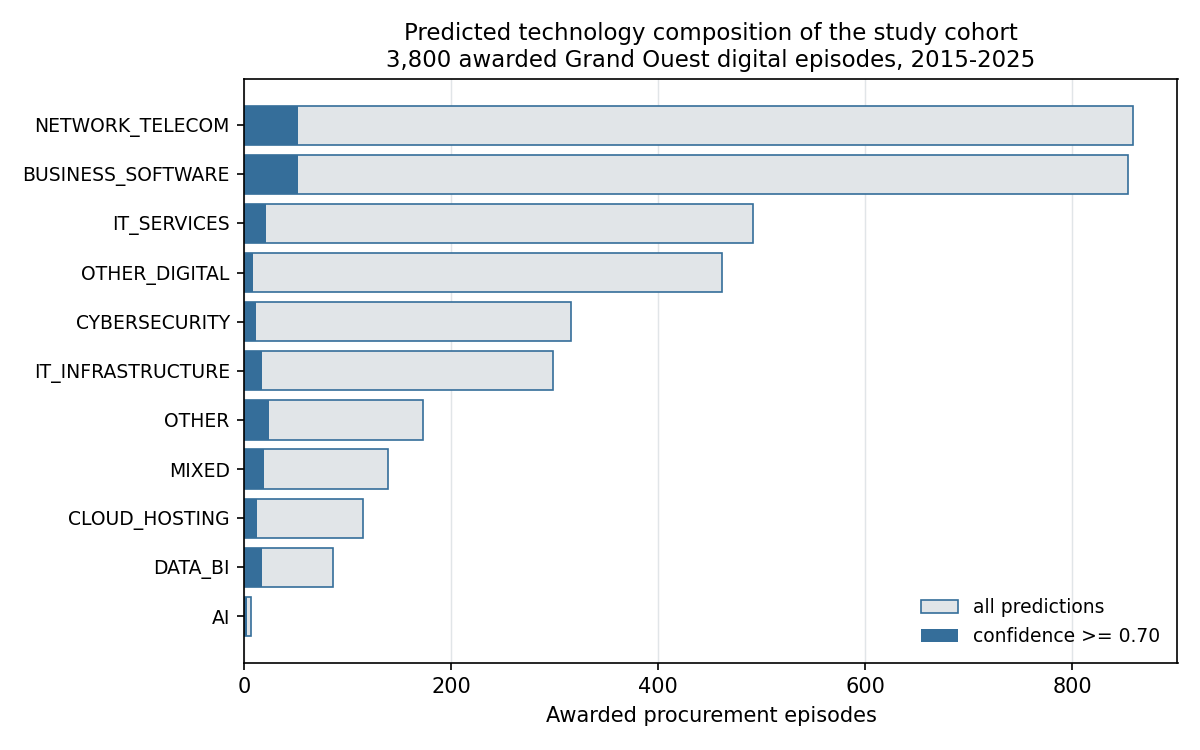
\includegraphics[width=0.85\linewidth]{figures/fig06_technology_composition.png}
\caption{Predicted technology composition of the 3,800 cohort episodes, with the share clearing the 0.70 confidence cutoff overlaid. \texttt{NETWORK\_TELECOM} and \texttt{BUSINESS\_SOFTWARE} dominate at almost identical size, while \texttt{AI} holds six episodes across eleven years. The dark portion is small everywhere, a reminder that the deployed confidence score is conservative. \textbf{These counts are predictions, not market shares.}}
\label{fig:techcomp}
\end{figure}
